% ==========================================================
% PneumoFusionNet — Term Project Report PART 2 (Trimester 8)
% IIT Guwahati | B.Sc. Data Science & AI
% Ashutosh Yadav (Roll: 23035010693)
% ==========================================================

\documentclass{article}
\usepackage{spconf,amsmath,amssymb,graphicx,hyperref}
\usepackage{booktabs,enumitem,needspace,tikz,xcolor,tcolorbox}
\usetikzlibrary{arrows.meta,positioning,fit,backgrounds}

\hypersetup{colorlinks=true,linkcolor=blue!70!black,
            citecolor=blue!70!black,urlcolor=teal}
\tcbuselibrary{skins}
\definecolor{successgrn}{RGB}{39,174,96}
\definecolor{alertred}{RGB}{192,57,43}

% ── Global spacing tightening ──────────────────────────────
\setlength{\parskip}{1.5pt}
\setlength{\topsep}{1pt}
\setlength{\partopsep}{0pt}
\setlength{\itemsep}{1pt}
\setlength{\textfloatsep}{6pt plus 2pt minus 2pt}
\setlength{\floatsep}{5pt plus 2pt minus 2pt}
\setlength{\intextsep}{5pt plus 2pt minus 2pt}
\setlength{\abovecaptionskip}{3pt}
\setlength{\belowcaptionskip}{1pt}

\def\x{{\mathbf x}}
\def\L{{\cal L}}

% ------------------------------------------------------------------
\title{PneumoFusionNet Part~2: Multimodal Pneumonia Detection\\
via CXR Image, Radiology Text, and WBC Fusion}

\name{Ashutosh Yadav (Roll Number: 23035010693)}

\address{
  Term Project Report Part~2 (Trimester 8)\\[0.2em]
  B.Sc.\ (Honours) Data Science and Artificial Intelligence\\
  Indian Institute of Technology Guwahati, India \quad
  \texttt{ashutosh@op.iitg.ac.in}
}

% ==========================================================
\begin{document}
\ninept
\maketitle

% ==========================================================
\begin{abstract}
This report is Part~2 of the PneumoFusionNet term project. In Part~1 we found
that an image-only DenseNet-121 trained on MIMIC-CXR chest X-rays stopped
improving at AUC\,$\approx$\,0.826, no matter how much we tuned the training.
The reason is simple: the X-ray alone cannot tell us how the patient's body
is responding to infection. To fix this, Part~2 adds two more sources of
information. In \textbf{Phase~2} we feed the radiology report text
(FINDINGS\,+\,HISTORY, with the diagnosis section removed to avoid cheating)
into Bio\_ClinicalBERT~\cite{alsentzer2019bert} and connect it to the image
through a cross-attention layer. This raises AUC to \textbf{0.949} and
Sensitivity to 91.4\%. In \textbf{Phase~3c}---the main focus of this report---we
add just one extra blood test result, the WBC count from a routine CBC that
is ready within 15 minutes of the patient arriving at the hospital.
This small addition pushes AUC to \textbf{0.971}, Sensitivity to \textbf{92.25\%},
and Specificity to \textbf{93.59\%} on a 3,763-image test set.
\textbf{Index Terms---} Chest X-Ray, Radiology Report, WBC, MIMIC-CXR,
Pneumonia Detection, Fusion Model.
\end{abstract}

\begin{keywords}
Pneumonia Detection, CXR, Radiology Text, WBC, Multimodal Fusion, MIMIC-CXR
\end{keywords}

% ==========================================================
\section{Introduction}
% ==========================================================

Pneumonia kills around 2.5 million people every year~\cite{who2023}, and the
chest X-ray is still the first thing a doctor orders when they suspect it.
The problem is that even experienced radiologists sometimes disagree on
whether a faint shadow on the image is pneumonia, fluid, or something else.
We started this project asking: can a computer help, and if so, what information
does it need beyond the X-ray?

Our Part~1 experiments showed that the X-ray image alone tops out at about
AUC\,=\,0.826. That ceiling exists because the image only shows what the lung
looks like---it cannot tell you whether the patient has a fever, how long they
have been sick, or whether their white blood cell count is elevated.
Two things that \emph{are} available in a real hospital setting can fill that gap.
First, the \textbf{radiology report}: when a radiologist reads the scan they write
a short paragraph about what they see (FINDINGS) and why the patient came in
(HISTORY). We use only these sections and always remove the final IMPRESSION
line, which states the diagnosis---letting the model read that would be cheating.
Second, the \textbf{WBC count}: a simple blood test that is part of every routine
CBC and comes back within 15 minutes of the patient arriving. A high WBC
is one of the earliest signs the body is fighting an infection.

In Part~2 we add these two pieces of information one at a time and measure
how much each one helps:
Phase~1 (X-ray only) $\to$
Phase~2 (X-ray\,+\,report text) $\to$
Phase~3c (X-ray\,+\,report text\,+\,WBC).
All experiments use the restricted MIMIC-CXR hospital dataset~\cite{johnson2019mimic}
(PhysioNet DUA and CITI ethics training required for access).

% ==========================================================
\section{Dataset}
% ==========================================================

We used \textbf{MIMIC-CXR-JPG~v2.0.0}~\cite{johnson2019mimic}, a large chest
X-ray dataset from Beth Israel Deaconess Medical Centre collected between
2011 and 2016. Access is restricted---you need to complete CITI ethics
training and sign a PhysioNet data agreement, which we did before starting.
We only kept \textbf{PA (front-on) views} because mixing in side or
bedridden-patient views confused earlier models in Part~1.
WBC counts were pulled from \textbf{MIMIC-IV}~\cite{johnson2023mimiciv}
lab records and matched to each X-ray by patient ID.
The full dataset has \textbf{3,763 images} (1,872 Normal, 1,891 Pneumonia,
roughly balanced), split by patient---never by image---so the same person
cannot appear in both training and testing:
Train~2,633 / Val~565 / Test~565.
About 15\% of WBC values were missing; we filled these with the median
value from the training set only and applied that same number to the
validation and test sets, so no test information leaks in.
In every case, the IMPRESSION section of the report was removed---that
section tells the reader the diagnosis, and the model should not see it.

% ==========================================================
\section{Architecture}
% ==========================================================

\subsection{Phase~1 --- X-Ray Only (Starting Point)}

We used DenseNet-121~\cite{huang2017densenet}, a well-known image network
pretrained on more than 500\,000 real chest X-rays through the
TorchXRayVision~\cite{cohen2022torchxrayvision} library. On top of it we
attached a CBAM~\cite{woo2018cbam} attention block that tells the network
which parts of the image to focus on. Training used 5-fold cross-validation
with Focal Loss~\cite{lin2017focal} ($\gamma$\,=\,2.0) to handle the cases
the model kept getting wrong. The features from the best fold (1024 numbers
summarising the image, kept frozen) are reused in Phases 2 and 3c.

\subsection{Phase~2 --- Adding the Radiology Report}

We fed the cleaned report text into
Bio\_ClinicalBERT~\cite{alsentzer2019bert}, a language model pretrained on
hospital notes. The last two layers were lightly fine-tuned (learning rate
1e-5) so it could adapt to our task without forgetting everything it learned.
Rather than just averaging the text into a single number, we used an
8-head cross-attention layer so the X-ray features could look at each word
of the report and decide which parts are most relevant:
\vspace{-2pt}
\begin{equation}
  \mathbf{c} = \mathrm{softmax}\!\left(\frac{\mathbf{Q}_{\mathrm{img}}
  \mathbf{K}_{\mathrm{txt}}^\top}{\sqrt{d_k}}\right)\mathbf{V}_{\mathrm{txt}},
  \quad d_k = 64
  \label{eq:crossattn}
\end{equation}
We trained with Focal Loss ($\gamma$\,=\,2.0) and Mixup~\cite{zhang2018mixup}
($\alpha$\,=\,0.2) on the combined embeddings, with the image-text head
learning at 2e-4 and BERT at the slower 1e-5 to keep it stable.

\subsection{Phase~3c --- Adding WBC (Main Model)}

\begin{figure}[t]
\centering
\resizebox{\columnwidth}{!}{%
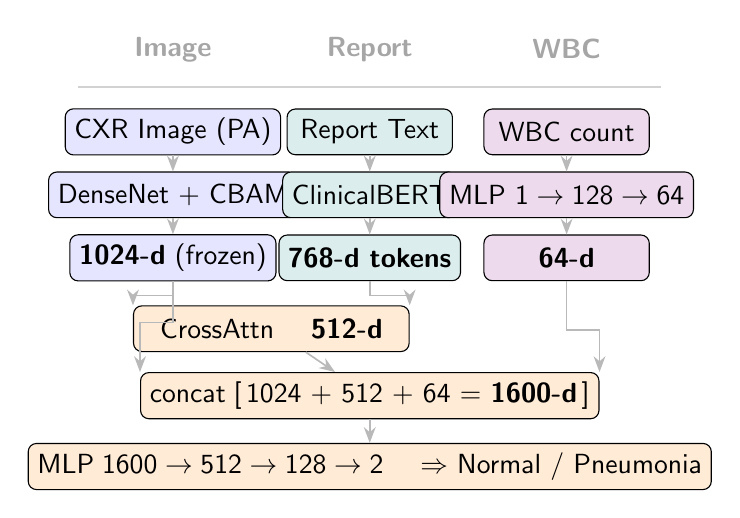
\begin{tikzpicture}[
  % ── Node styles ──────────────────────────────────────
  hdr/.style   ={font=\normalsize\bfseries\sffamily, text=gray!70},
  imgbox/.style={draw, rounded corners=3pt, fill=blue!10,
                 minimum height=0.58cm, minimum width=2.1cm,
                 align=center, font=\normalsize\sffamily},
  txtbox/.style={draw, rounded corners=3pt, fill=teal!14,
                 minimum height=0.58cm, minimum width=2.1cm,
                 align=center, font=\normalsize\sffamily},
  wbcbox/.style={draw, rounded corners=3pt, fill=violet!14,
                 minimum height=0.58cm, minimum width=2.1cm,
                 align=center, font=\normalsize\sffamily},
  fusbox/.style={draw, rounded corners=3pt, fill=orange!16,
                 minimum height=0.58cm, align=center,
                 font=\normalsize\sffamily},
  arr/.style   ={-Stealth, semithick, gray!55}
]

% ── Column headers (y = 5.2, well above top boxes at y = 4.0) ──
\node[hdr] at (0,   5.2) {Image};
\node[hdr] at (2.5, 5.2) {Report};
\node[hdr] at (5.0, 5.2) {WBC};

% ── Horizontal separator line ────────────────────────────────────
\draw[gray!35, thin] (-1.2, 4.72) -- (6.2, 4.72);

% ── Image branch  (x = 0) ────────────────────────────────────────
\node[imgbox](img)  at (0, 4.15) {CXR Image (PA)};
\node[imgbox](dn)   at (0, 3.35) {DenseNet + CBAM};
\node[imgbox](iemb) at (0, 2.55) {\textbf{1024-d} (frozen)};

% ── Text branch   (x = 2.5) ──────────────────────────────────────
\node[txtbox](rep)  at (2.5, 4.15) {Report Text};
\node[txtbox](bert) at (2.5, 3.35) {ClinicalBERT};
\node[txtbox](temb) at (2.5, 2.55) {\textbf{768-d tokens}};

% ── WBC branch    (x = 5.0) ──────────────────────────────────────
\node[wbcbox](wbc1) at (5.0, 4.15) {WBC count};
\node[wbcbox](wbc2) at (5.0, 3.35) {MLP 1\;$\to$\;128\;$\to$\;64};
\node[wbcbox](wbc3) at (5.0, 2.55) {\textbf{64-d}};

% ── Fusion layer ─────────────────────────────────────────────────
\node[fusbox, minimum width=3.5cm](ca)
      at (1.25, 1.65) {CrossAttn \quad \textbf{512-d}};

\node[fusbox, minimum width=5.8cm](cc)
      at (2.5,  0.80) {concat\;[\,1024 + 512 + 64 = \textbf{1600-d}\,]};

\node[fusbox, minimum width=5.8cm](cls)
      at (2.5, -0.10) {MLP\;1600\;$\to$\;512\;$\to$\;128\;$\to$\;2
                       \quad $\Rightarrow$ Normal / Pneumonia};

% ── Arrows ───────────────────────────────────────────────────────
\draw[arr](img)--(dn);    \draw[arr](dn)--(iemb);
\draw[arr](rep)--(bert);  \draw[arr](bert)--(temb);
\draw[arr](wbc1)--(wbc2); \draw[arr](wbc2)--(wbc3);

\draw[arr](iemb.south)--++(0,-0.18)-|(ca.north west);
\draw[arr](temb.south)--++(0,-0.18)-|(ca.north east);
\draw[arr](ca)--(cc);
\draw[arr](iemb.south)--++(0,-0.52)-|(cc.north west);
\draw[arr](wbc3.south)--++(0,-0.62)-|(cc.north east);
\draw[arr](cc)--(cls);

\end{tikzpicture}%
}
\vspace{-2pt}
\caption{Phase~3c model. Three inputs---chest X-ray, leakage-free report text,
and WBC blood count---flow through separate branches, join via cross-attention
and concatenation, then go to a small classifier (Normal / Pneumonia).}
\label{fig:p3c}
\end{figure}

The WBC count is just one number, but we did not pass it in raw.
A small three-layer network ($1\!\to\!128\!\to\!128\!\to\!64$) turns it into
64 numbers first, because a WBC of 12 vs.\ 15 vs.\ 25\,K/\textmu{}L
mean very different things clinically (borderline / high / very high),
and a raw number cannot capture that difference.
The three branches are then joined together:
\vspace{-2pt}
\begin{equation}
  \mathbf{z} = [\,\mathbf{v}_{\mathrm{img}} \,\|\,
  \mathbf{c}_{\mathrm{cross}} \,\|\, \mathbf{e}_{\mathrm{wbc}}\,]
  \in \mathbb{R}^{1600}
  \label{eq:p3c}
\end{equation}
We loaded the Phase~2 cross-attention weights as the starting point
so the model did not have to learn the image-text part from scratch again.
Learning rates: BERT\,=\,1e-5, fusion head\,=\,2e-4, WBC network\,=\,1e-3.


% ==========================================================
\section{Conclusion}
% ==========================================================

\begin{enumerate}[noitemsep,leftmargin=*,topsep=3pt]

  \item \textbf{The X-ray alone was not enough.}
    Even our best image-only model stopped improving at AUC\,=\,0.826.
    The lung picture shows the damage but not the body's response to it.

  \item \textbf{Adding the radiology report made the biggest difference.}
    Once we included the FINDINGS and HISTORY text (with IMPRESSION removed),
    AUC jumped to \textbf{0.949} and the model started catching 91\% of
    pneumonia cases---a gain of more than 12 percentage points in AUC.

  \item \textbf{One blood test made it even better.}
    Adding just the WBC count pushed AUC to \textbf{0.971} and sensitivity
    to \textbf{92.3\%}. That is better sensitivity than the full 17-lab-test
    model, while needing only one result that is ready in 15 minutes.

  \item \textbf{This is practical in a real hospital.}
    A doctor in the emergency room gets the chest X-ray done, the radiologist
    writes a brief report, and the CBC comes back---all within 30 minutes.
    Our model needs nothing more than these three things to give a
    reliable second opinion on whether the patient has pneumonia.

  \item \textbf{Next step --- test this on Indian patient data.}
    Everything so far used data from a US hospital (MIMIC-CXR).
    For the next phase we plan to work with chest X-ray images and WBC
    values collected from Indian hospitals. The patient population is
    different---TB is common, malnutrition affects X-ray patterns,
    and the scanners and reporting styles vary a lot from Western centres.
    We want to check whether the X-ray\,+\,WBC model still works well
    on this data, and if not, fine-tune it so that it does.
    This will be a more honest test of whether the approach can actually
    help in the Indian clinical setting.

\end{enumerate}

\noindent\textbf{Code and results:}
\href{https://github.com/Ashutosh-yadav0001/PneumoFusionNet}%
{\texttt{github.com/Ashutosh-yadav0001/PneumoFusionNet}}.
Phase~3c notebook: \texttt{Phase-3c-wbc\_only\_fusion.ipynb} in
\texttt{mimic/main/Phase-3/}.
MIMIC-CXR data is restricted (PhysioNet DUA and CITI required).




% ==========================================================
\small
\begin{thebibliography}{9}

\bibitem{pneumofusionnet_part1}
A.~Yadav, ``PneumoFusionNet Part~1: Data Preparation and Pilot Experiments,''
\emph{Term Project Report (Trimester~8)}, IIT Guwahati, 2026.

\bibitem{frontiers2025pneumofusion}
S.~Yu et al., ``A multi-modal deep learning solution for precise pneumonia
diagnosis: the PneumoFusion-Net model,'' \emph{Frontiers in Physiology},
vol.~16, Art.~1512835, Mar.\ 2025.

\bibitem{rajpurkar2017chexnet}
P.~Rajpurkar et al., ``CheXNet: Radiologist-Level Pneumonia Detection on Chest
X-Rays with Deep Learning,'' \emph{arXiv:1711.05225}, 2017.

\bibitem{johnson2019mimic}
A.~E.~W.~Johnson et al., ``MIMIC-CXR, a de-identified publicly available
database of chest radiographs with free-text reports,''
\emph{Scientific Data}, vol.~6, no.~317, 2019.

\bibitem{johnson2023mimiciv}
A.~E.~W.~Johnson et al., ``MIMIC-IV, a freely accessible electronic health
record dataset,'' \emph{Scientific Data}, vol.~10, no.~1, p.~1, 2023.

\bibitem{alsentzer2019bert}
E.~Alsentzer et al., ``Publicly Available Clinical BERT Embeddings,''
\emph{arXiv:1904.03323}, 2019.

\bibitem{huang2017densenet}
G.~Huang, Z.~Liu, L.~van~der~Maaten, and K.~Q.~Weinberger,
``Densely Connected Convolutional Networks,''
\emph{Proc.\ IEEE CVPR}, 2017, pp.~4700--4708.

\bibitem{woo2018cbam}
S.~Woo, J.~Park, J.-Y.~Lee, and I.~S.~Kweon,
``CBAM: Convolutional Block Attention Module,''
\emph{Proc.\ ECCV}, 2018, pp.~3--19.

\bibitem{lin2017focal}
T.-Y.~Lin, P.~Goyal, R.~Girshick, K.~He, and P.~Doll{\'a}r,
``Focal Loss for Dense Object Detection,''
\emph{Proc.\ IEEE ICCV}, 2017, pp.~2980--2988.

\bibitem{zhang2018mixup}
H.~Zhang, M.~Ciss{\'e}, Y.~N.~Dauphin, and D.~Lopez-Paz,
``Mixup: Beyond Empirical Risk Minimization,''
\emph{Proc.\ ICLR}, 2018.

\bibitem{cohen2022torchxrayvision}
J.~P.~Cohen et al.,
``TorchXRayVision: A Library of Chest X-Ray Datasets and Models,''
\emph{Proc.\ MICCAI Workshop on Medical Imaging with Deep Learning}, 2022.

\bibitem{who2023}
World Health Organization, ``Pneumonia,'' \emph{WHO Fact Sheet}, 2023.
\url{https://www.who.int/news-room/fact-sheets/detail/pneumonia}

\end{thebibliography}

\end{document}
